\section{The Modelling Layer}
\label{sec:modelling_layer}

The first layer to be described of the AdaptUI architecture is the Modelling
Layer. This layer aims to generate the different profiles (semantic models) for
the three main entities: the user, the current context and the device. In order
to do this, the Modelling Layer combines the results of two different modules: 
the Capabilities Collector and the Semantic Modeller. The Capabilities Collector
collects information about the three main entities. This module deals with the
current capabilities of the user, the environment current situation, and with
several characteristics of the device, storing the collected information for
further usage. On the other hand, the Semantic Modeller represents the knowledge
gathered and stored by the Capabilities Collector in a semantic model specified
at the AdaptUIOnt ontology (which is fully described in 
Chapter~\ref{cha:ontology_model}). 

The two modules which form the Modelling Layer are described in the following
sections. First, the Capabilities Collector is introduced in
Section~\ref{sec:capabilities_collector}. Next, the Semantic Modeller is
presented in Section~\ref{sec:semantic_modeller}.


\subsection{The Capabilities Collector}
\label{sec:capabilities_collector}

As mentioned in the literature, \citet{fischer_user_2001} defended that the user
evolves through time. More concretely, time and experience are two of the 
reasons for the  evolution of user's characteristics. In AdaptUI users 
evolve, but under different assumptions. Fischer considered long terms 
parameters as the keys for the evolution of the user. On the contrary, AdaptUI 
takes into account temporary and concrete context conditions, limited to a 
specific momentum. Consequently, the user model is built contemplating a dynamic 
user whose capabilities change due to context conditions.

Considering this dynamic user perspective based on several aspects related to
context terms, we discussed how this could be applicable to mobile devices. 
Mobile devices have several characteristics that make them susceptible to change 
(i.e., battery consumption, location awareness, preferences of the screen or 
sound). Thus, in AdaptUI mobile devices are also considered as a dynamic entity.

Finally, regarding the surrounding environment, we consider that it also has the 
propensity to change (i.e., temperature, light or noise). Therefore, within the 
Modelling Layer a concrete module to collect these characteristics has been 
designed: the Capabilities Collector.

The Capabilities Collector is a software module that allows the system gathering 
non physiological capabilities of the user, collect different variables of the 
current environment situation, and identify several device characteristics in 
order to be aware of the whole domain limitations. Figure~\ref{fig:capabilities_collector_flow}
illustrates how the Capabilities Collector uses several activities to collect
the information about the three entities. This information is transferred to the
Semantic Modeller.

\begin{figure}
\centering
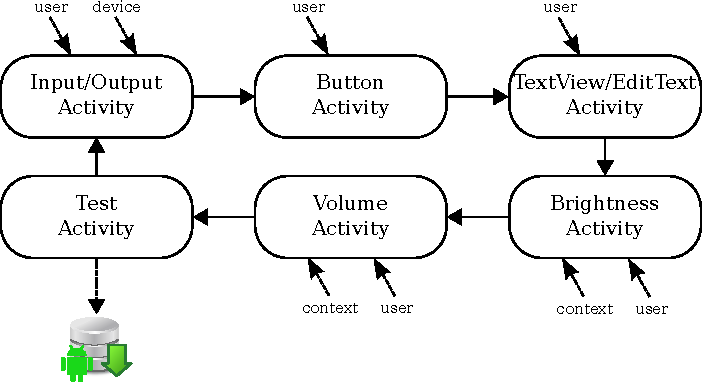
\includegraphics[width=0.65\textwidth]{capabilities_collector_flow.pdf}
\caption{The Capabilities Collector activities and their relationships with the
three main entities in AdaptUI.}
\label{fig:capabilities_collector_flow}
\end{figure}


\subsubsection{Android Activity}
\label{sec:activities}

In Android, activities~\citep{activities}
are application components that provide a screen with which the user can interact.
Each activity is given a window in which to draw its user interface. Android
applications usually consist of multiple activities that bound to each other. 

Android applications have to declare a Main activity. This activity is always
presented to the user when launching the application for the first time. Besides,
activities can start other activities storing their current status (if needed).
An activity lifecycle is illustrated in Figure~\ref{fig:activity_lifecycle}.

\begin{figure}[H]
\centering
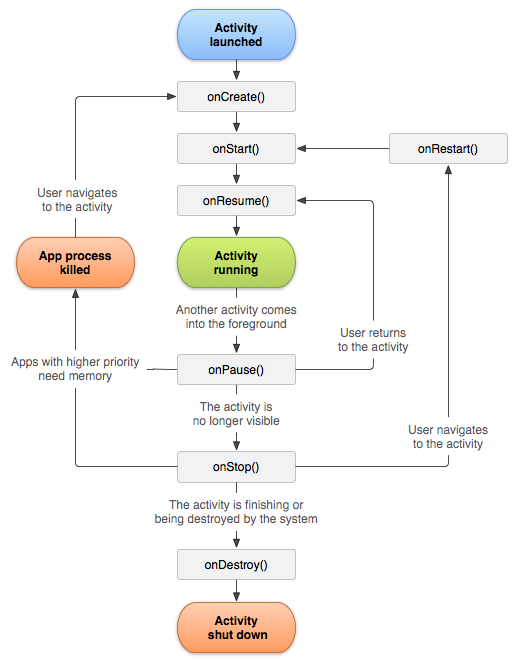
\includegraphics[width=0.55\textwidth]{activity_lifecycle.png}
\caption{The activity lifecycle.}
\label{fig:activity_lifecycle}
\end{figure}

To create an activity the developer has to extend the Activity class. A main
callback method is needed to be implemented: the \textit{onCreate()} method.
The system always calls this method when creating an activity. In it, the
essential components of the activity should be initialized. Besides, and before
any initialization, the \textit{setContentView()} method has to be called. This
method defines the layout for the activity's user interface, which is defined as
an \ac{xml} file in the \textit{layout} folder of the Android project.

Listing~\ref{lst:android_activity} shows an example of an activity initialization.
The layout of the activity is shown in Listing~\ref{lst:activity_layout}. Next,
Figure~\ref{fig:android_activity} illustrates the result of such activity.

\inputminted[linenos=true, fontsize=\footnotesize, frame=lines]{java}{4_system_architecture/android_activity.java}
\captionof{listing}{Example of an activity initialized with a button.\label{lst:android_activity}}

\inputminted[linenos=true, fontsize=\footnotesize, frame=lines]{xml}{4_system_architecture/activity_layout.xml}
\captionof{listing}{An activity layout declaring a button.\label{lst:activity_layout}}

\begin{figure}
\centering
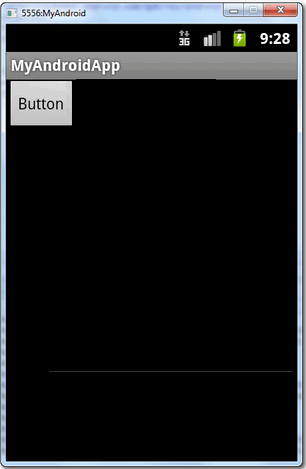
\includegraphics[width=0.35\textwidth]{android_activity.png}
\caption{The resulting activity from the combination of Listing~\ref{lst:android_activity},
Listing~\ref{lst:activity_layout} and Listing~\ref{lst:android_manifest}.}
\label{fig:android_activity}
\end{figure}

It is also important to remember defining the activity in the \textit{AndroidManifest.xml}
file. This file gathers the main specification of the declared activities, filters,
services and allowed permissions, along with the identification of the application.
Listing~\ref{lst:android_manifest} shows an example of a typical manifest file.

\inputminted[linenos=true, fontsize=\footnotesize, frame=lines]{xml}{4_system_architecture/android_manifest.xml}
\captionof{listing}{Application manifest file.\label{lst:android_manifest}}

\subsubsection{Collecting the User's Capabilities}
\label{sec:user_capabilities}

AdaptUI requires the user's capabilities (together with the current context
situation and the characteristics of the mobile device) as an input  for the
adaptation process. As explained in Section~\ref{sec:entities_model}, the user
model of the AdaptUIOnt model does not consider physiological knowledge about
the user. This is due to the lack of physiological and medical background that
users (and developers) of AdaptUI might have, which makes the capabilities
representation inaccurate and impractical. Instead of this, the user model
within the AdaptUIOnt ontology provides a layer of abstraction, focusing on the
user interaction needs. For example, a user who suffers from a hearing disability
in AdaptUI can explicitly configure a minimum sound level, so the system will
not reduce it in any future adaptation. Thus, we avoid modelling specific
physiological problems related to the user's hearing capability. To collect this
kind of information about the user, the Capabilities Collector shows several
screens (known as activities in Android) to the user in which different
interactions are required. 

The first capability that the Capabilities Collector deals with is the input
method or type of interaction. In the AdaptUIOnt ontology this is represented
through the \textit{Interface} class. Through several basic instructions
(presented in text mode and as quick audio question) the user selects his/her
input and output preferences. For example, Figure~\ref{fig:input_activity} shows
the first activity of the Capabilities Collector module. The instructions shown
in this activity can be read by the user and by the application itself (for
example, by using the Android \ac{tts}~\citep{tts} service). Every decision
the user makes is stored in the mobile phone as a profile for a future
\textit{semantization} by the Semantic Modeller.

\begin{figure}
\centering
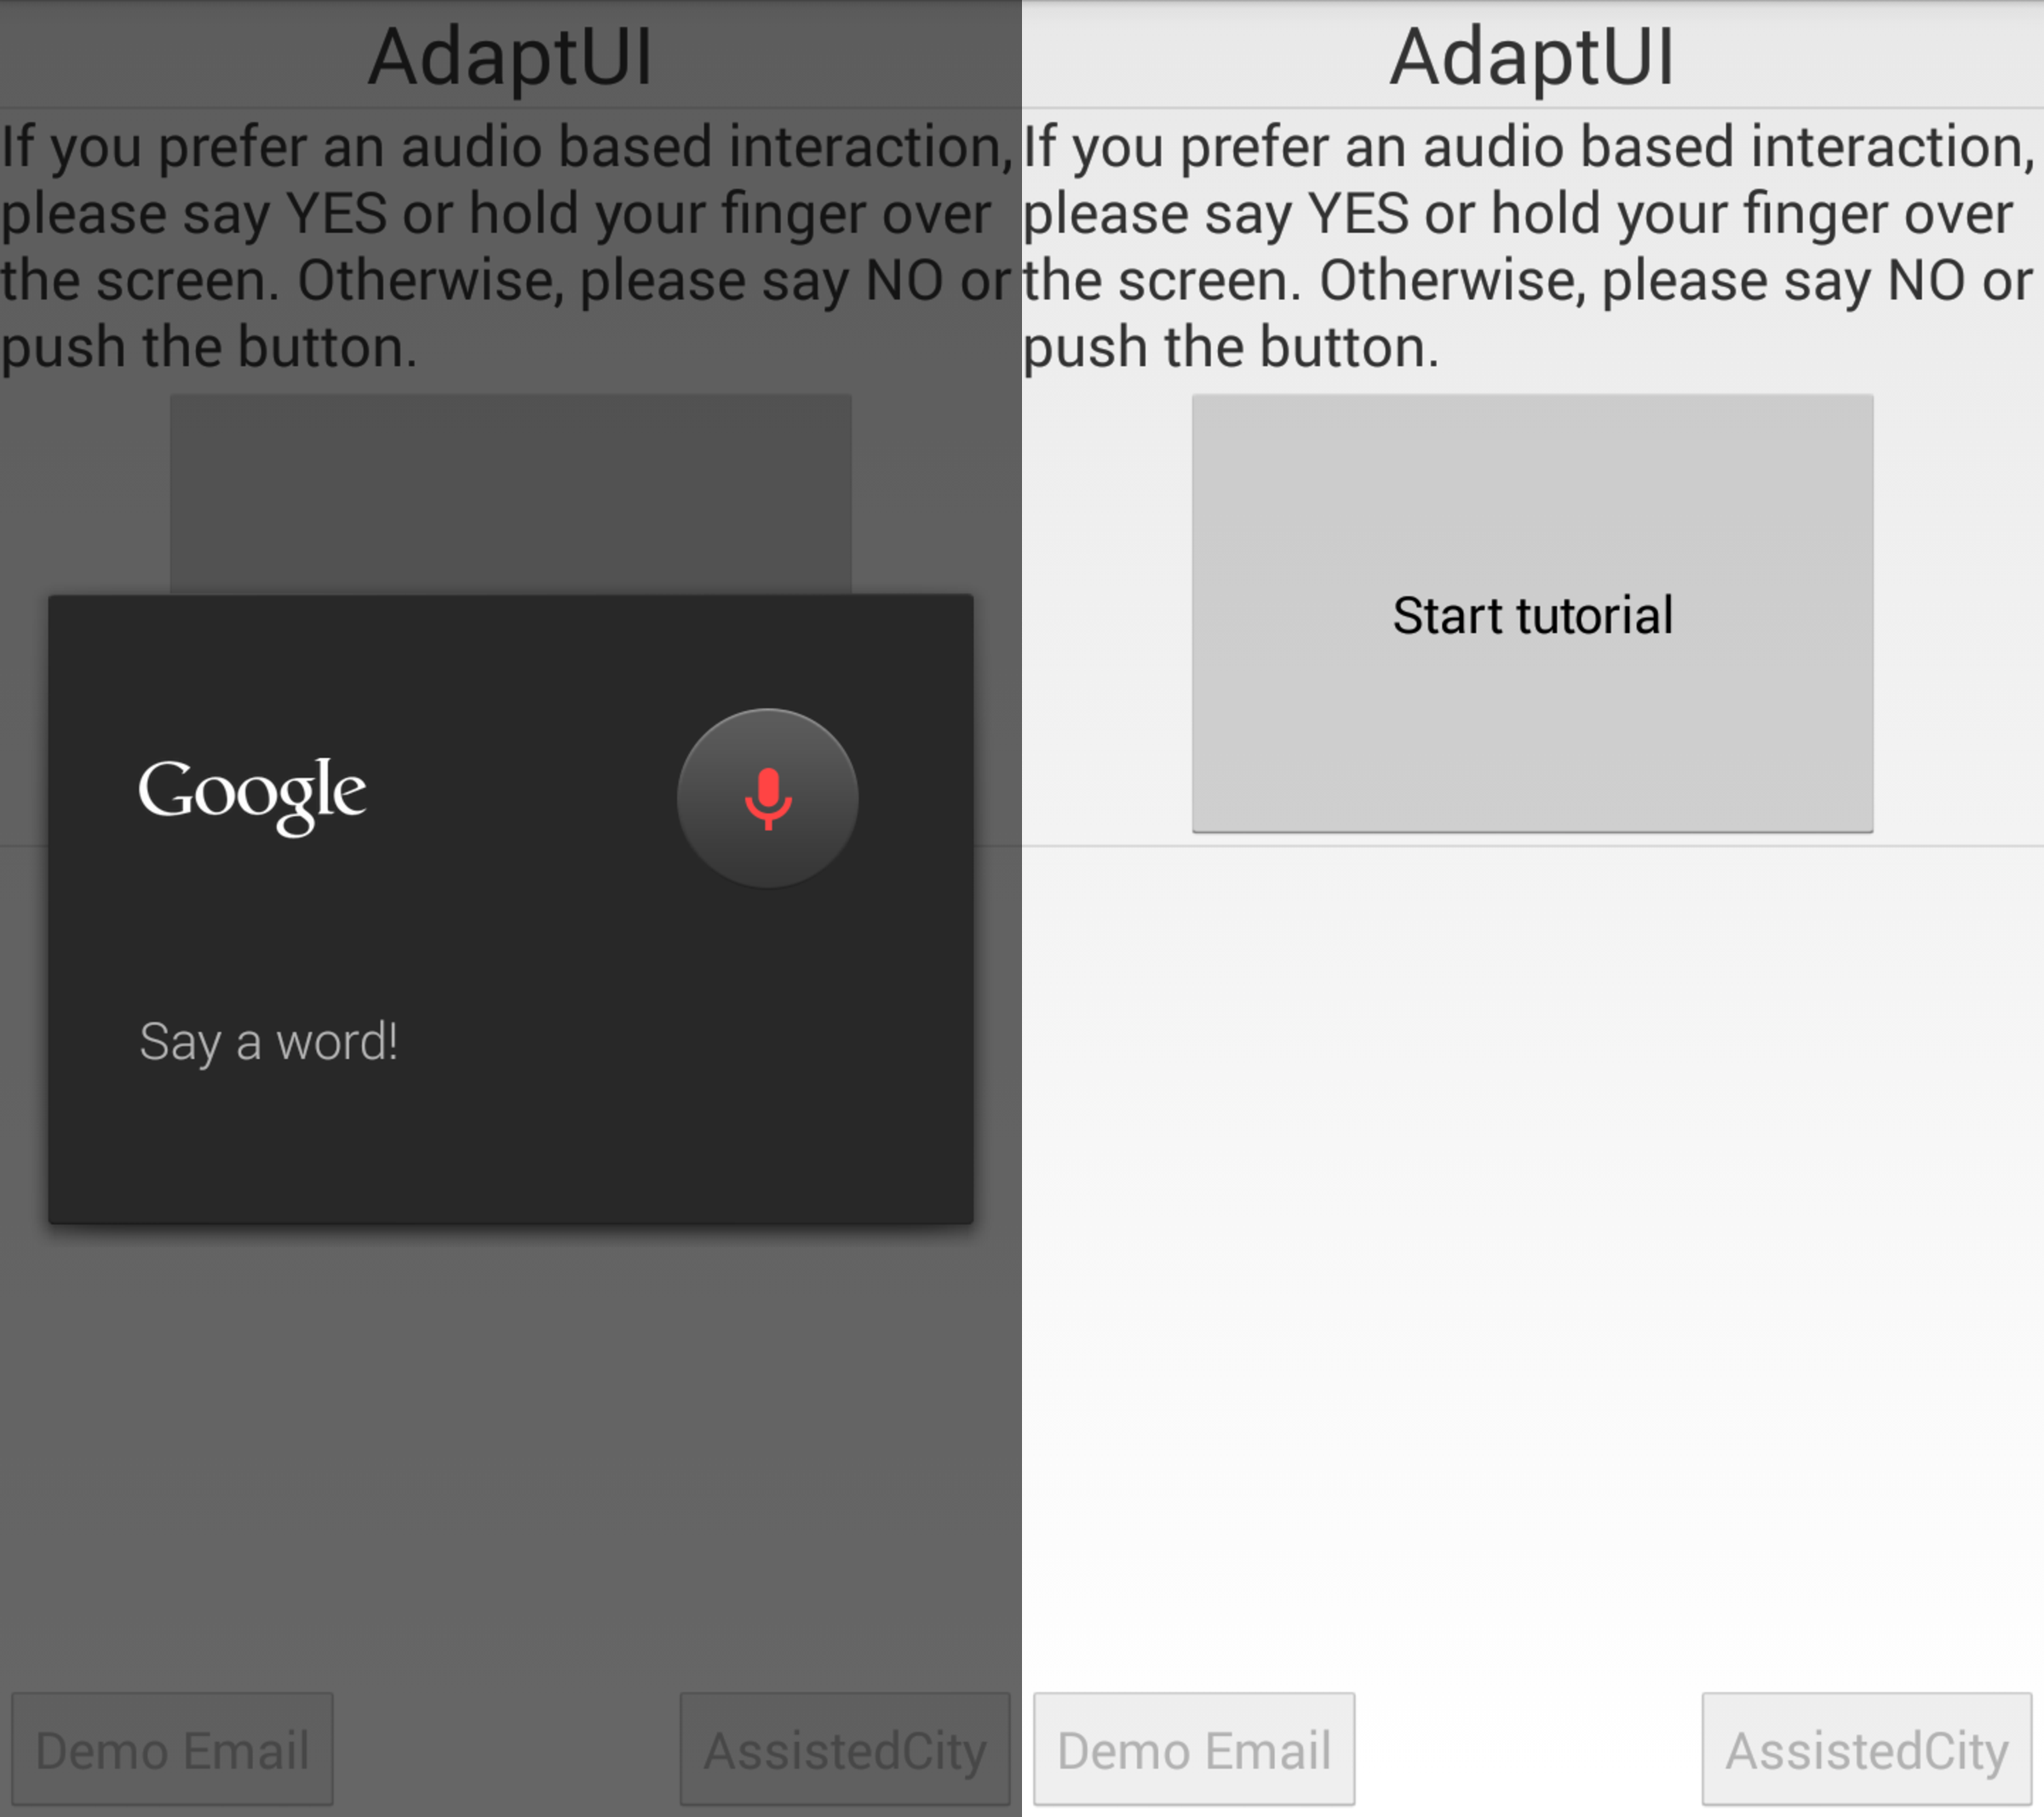
\includegraphics[width=0.50\textwidth]{input_activity.pdf}
\caption{Capabilities Collector's input activity.}
\label{fig:input_activity}
\end{figure}

Once the input interaction type has been determined the output is configured 
accordingly. Next activities show several Android view~\citep{android_view} 
components which are configurable by the user. Views represent the basic 
building block for user interface components in Android. A view occupies a 
particular area on the screen and is responsible for drawing and event 
handling. In this case, a button, a text view and an 
edit text (which is a particular case of a text view) are presented (see 
Figure~\ref{fig:views_activity}). The Capabilities Collector allows the user to 
modify their size, component colour, and also the text size and colour.

\begin{figure}
\centering
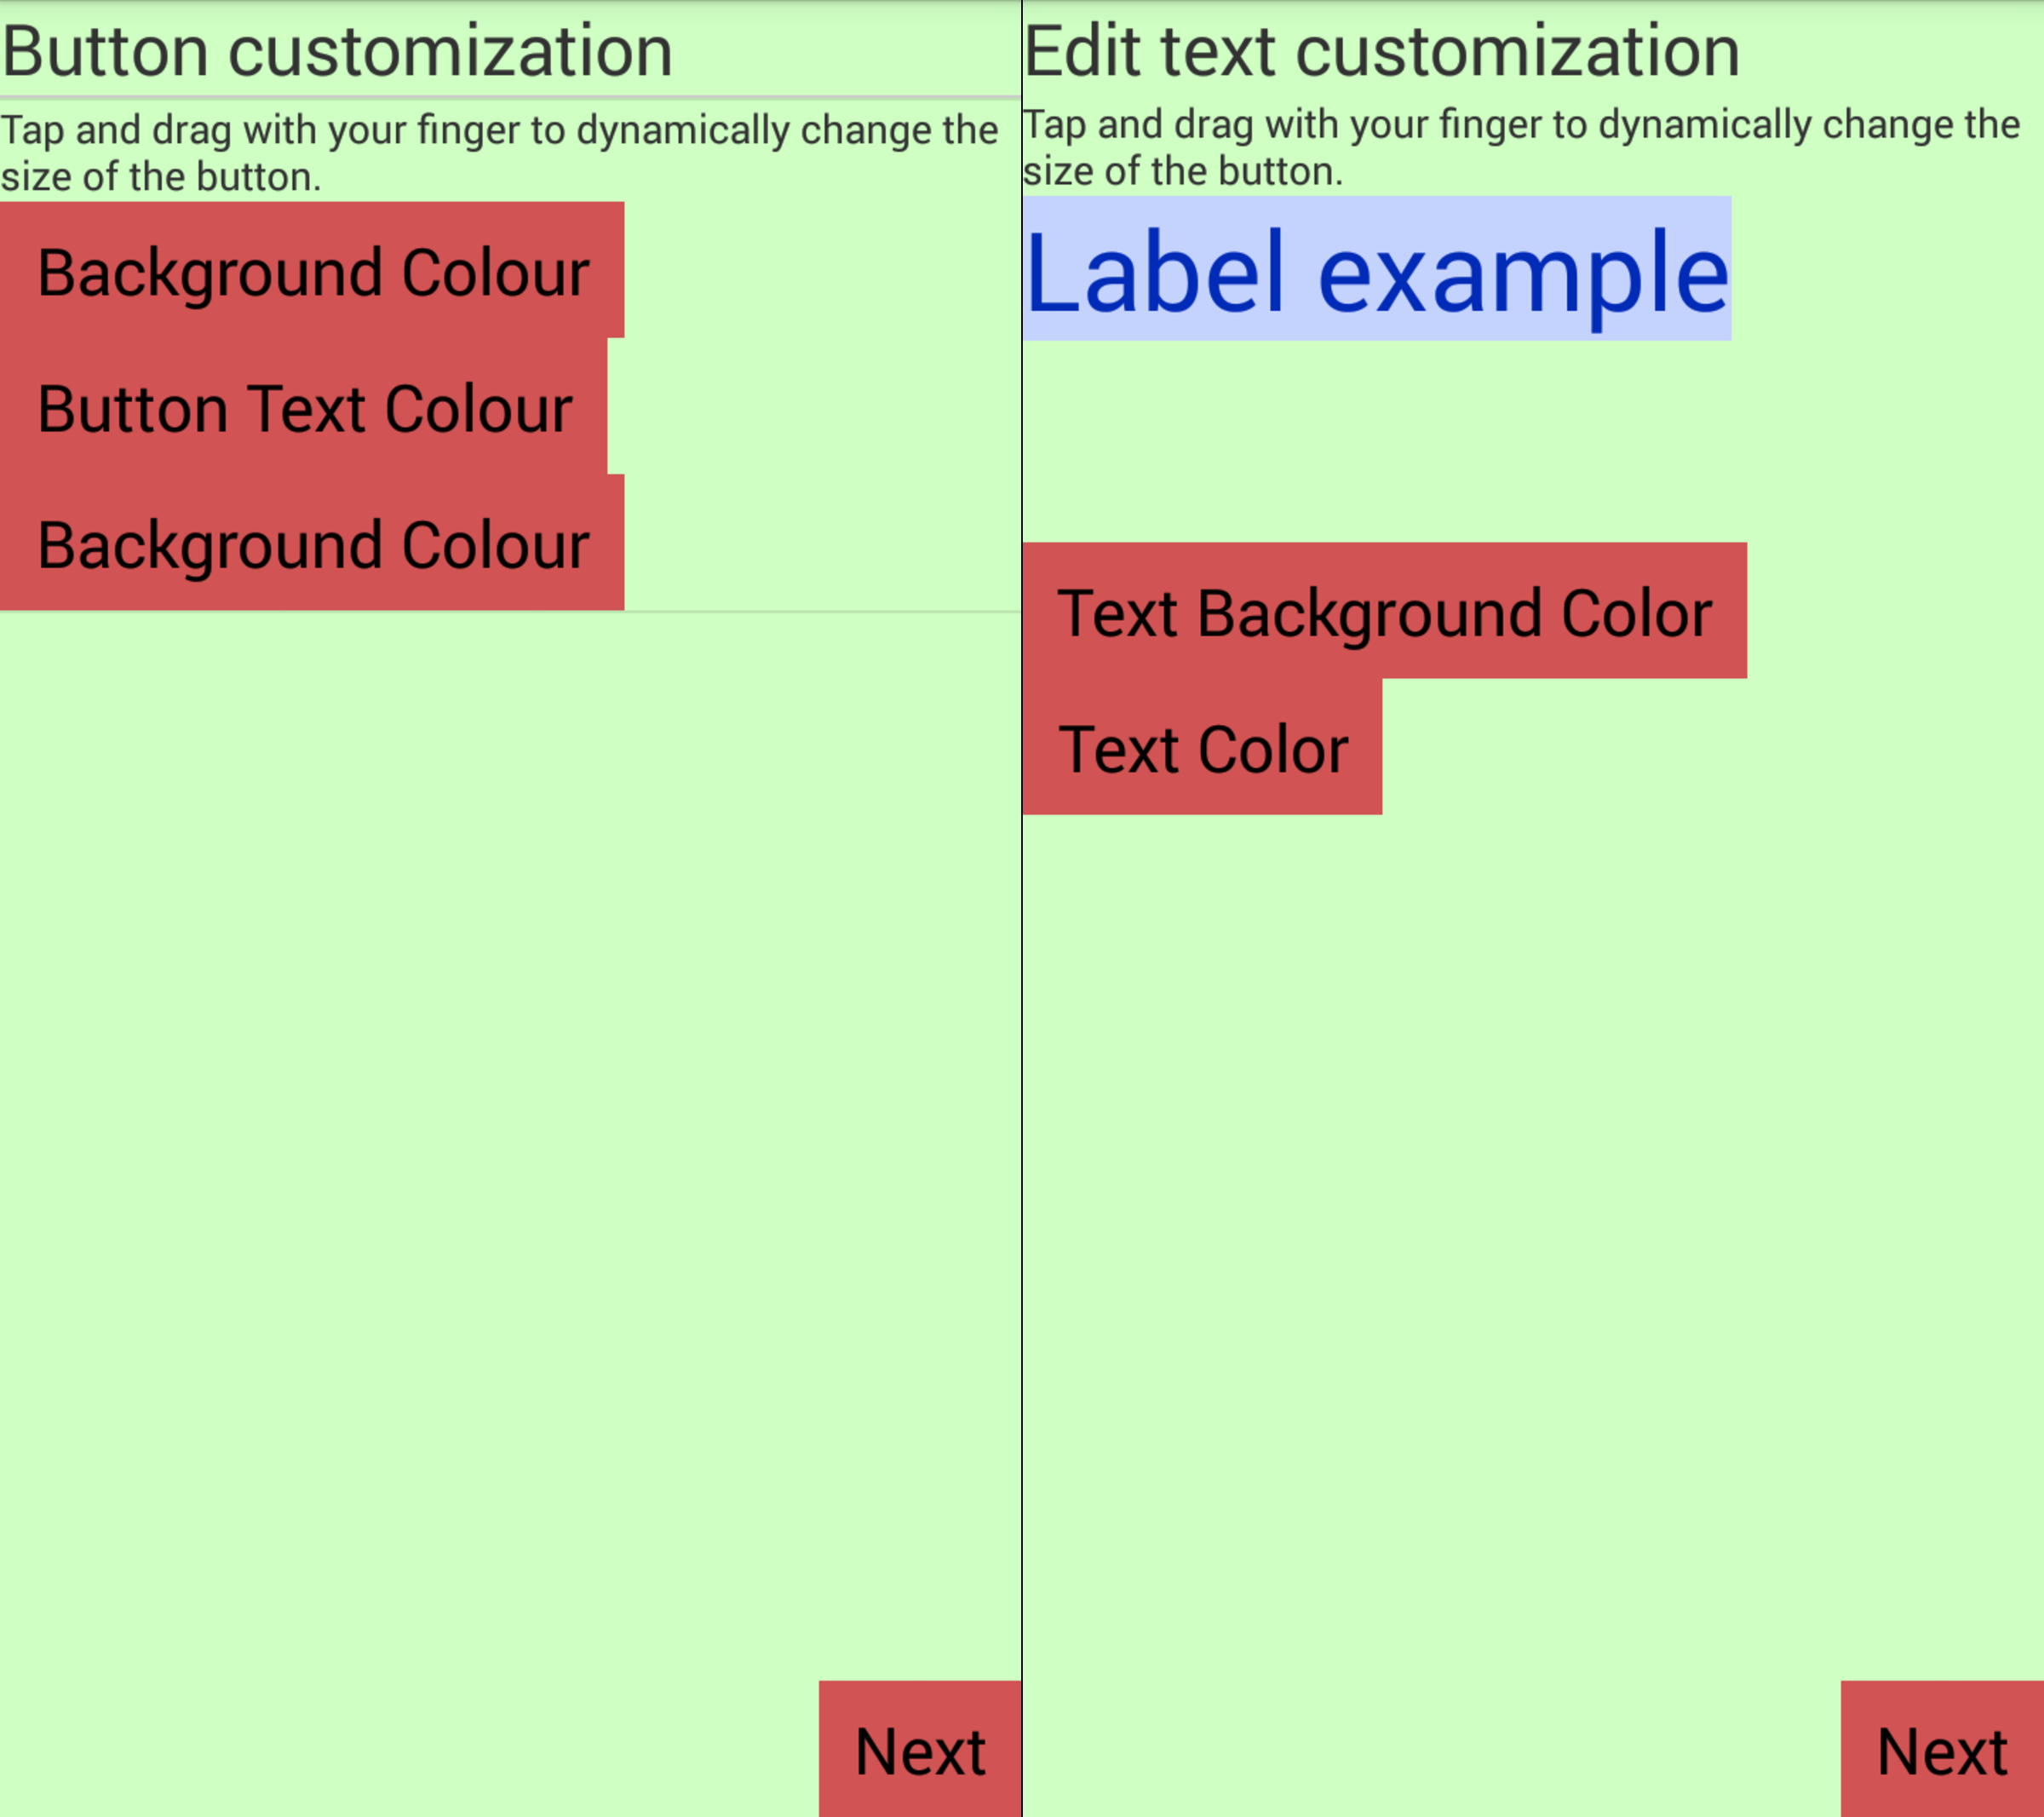
\includegraphics[width=0.50\textwidth]{views_activity.pdf}
\caption{Different Android view components
personalization: on the left, button; on the right, text view and edit text.}
\label{fig:views_activity}
\end{figure}

Finally, the display brightness and the system volume are also allowed to be
customized. The surrounding light and noise are monitored using the available
device sensors, which are listed by the Capabilities Collector when it is first
launched. Thus, AdaptUI is aware of the context conditions and is able to adjust
these parameters to the user's preferences.

 
\subsubsection{The Context Situation}
\label{sec:context_situation}
Current smartphones are equipped with several sensors that allow devices to
collect different environment parameters. Light sensors, microphones, proximity 
sensors for disabling the screen, even Bluetooth and infra-red transceivers are 
just several examples of the hardware available in such devices.

Taking advantage of the current situation, in which smartphones are able to sense
the environment, the Capabilities Collector collects knowledge of the user context.
Light conditions and noise are classified by the Capabilities Collector as follows:

\begin{itemize}
 \item Light conditions are measured in \ac{lx}, which is the \ac{si} unit of 
 luminance~\citep{lux}.
 
 \item The current noise is collected using the mobile available microphones. It
 is measured in \ac{db}, which is a logarithmic unit that expresses the ratio
 between two values of a physical quantity (often power or intensity).
\end{itemize}

Once all this features have been collected, the profile is temporarily stored in 
the device. This storage is carried out using the Android 
SharedPreferences~\citep{shared_preferences}.
This class provides a general persistence framework for developers to save and
retrieve key-value pairs of primitive data types. After this temporary storage
in the device, the Semantic Modeller is the module which deals with the task of
the semantic representation of the model. Listing~\ref{lst:shared_preferences}
shows how developers deal with the SharedPreferences to store and retrieve data
in Android. If complex objects are used, the process is different (see
Listing~\ref{lst:shared_preferences_complex}).

\inputminted[linenos=true, fontsize=\footnotesize, frame=lines]{java}{4_system_architecture/shared_preferences.java}
\captionof{listing}{Using Android SharedPreferences. By default SharedPreferences allows 
to store and retrieve primitive data. Implementing Parcelable allows complex 
objects to be persistent.\label{lst:shared_preferences}}

\inputminted[linenos=true, fontsize=\footnotesize, frame=lines]{java}{4_system_architecture/shared_preferences_complex.java}
\captionof{listing}{Using Android SharedPreferences to store non-primitive
objects.\label{lst:shared_preferences_complex}}

Figure~\ref{fig:context_activity} shows how the brightness and the volume of
the application is configured by a user which is aware of the light and noise
of the environment.

\begin{figure}
\centering
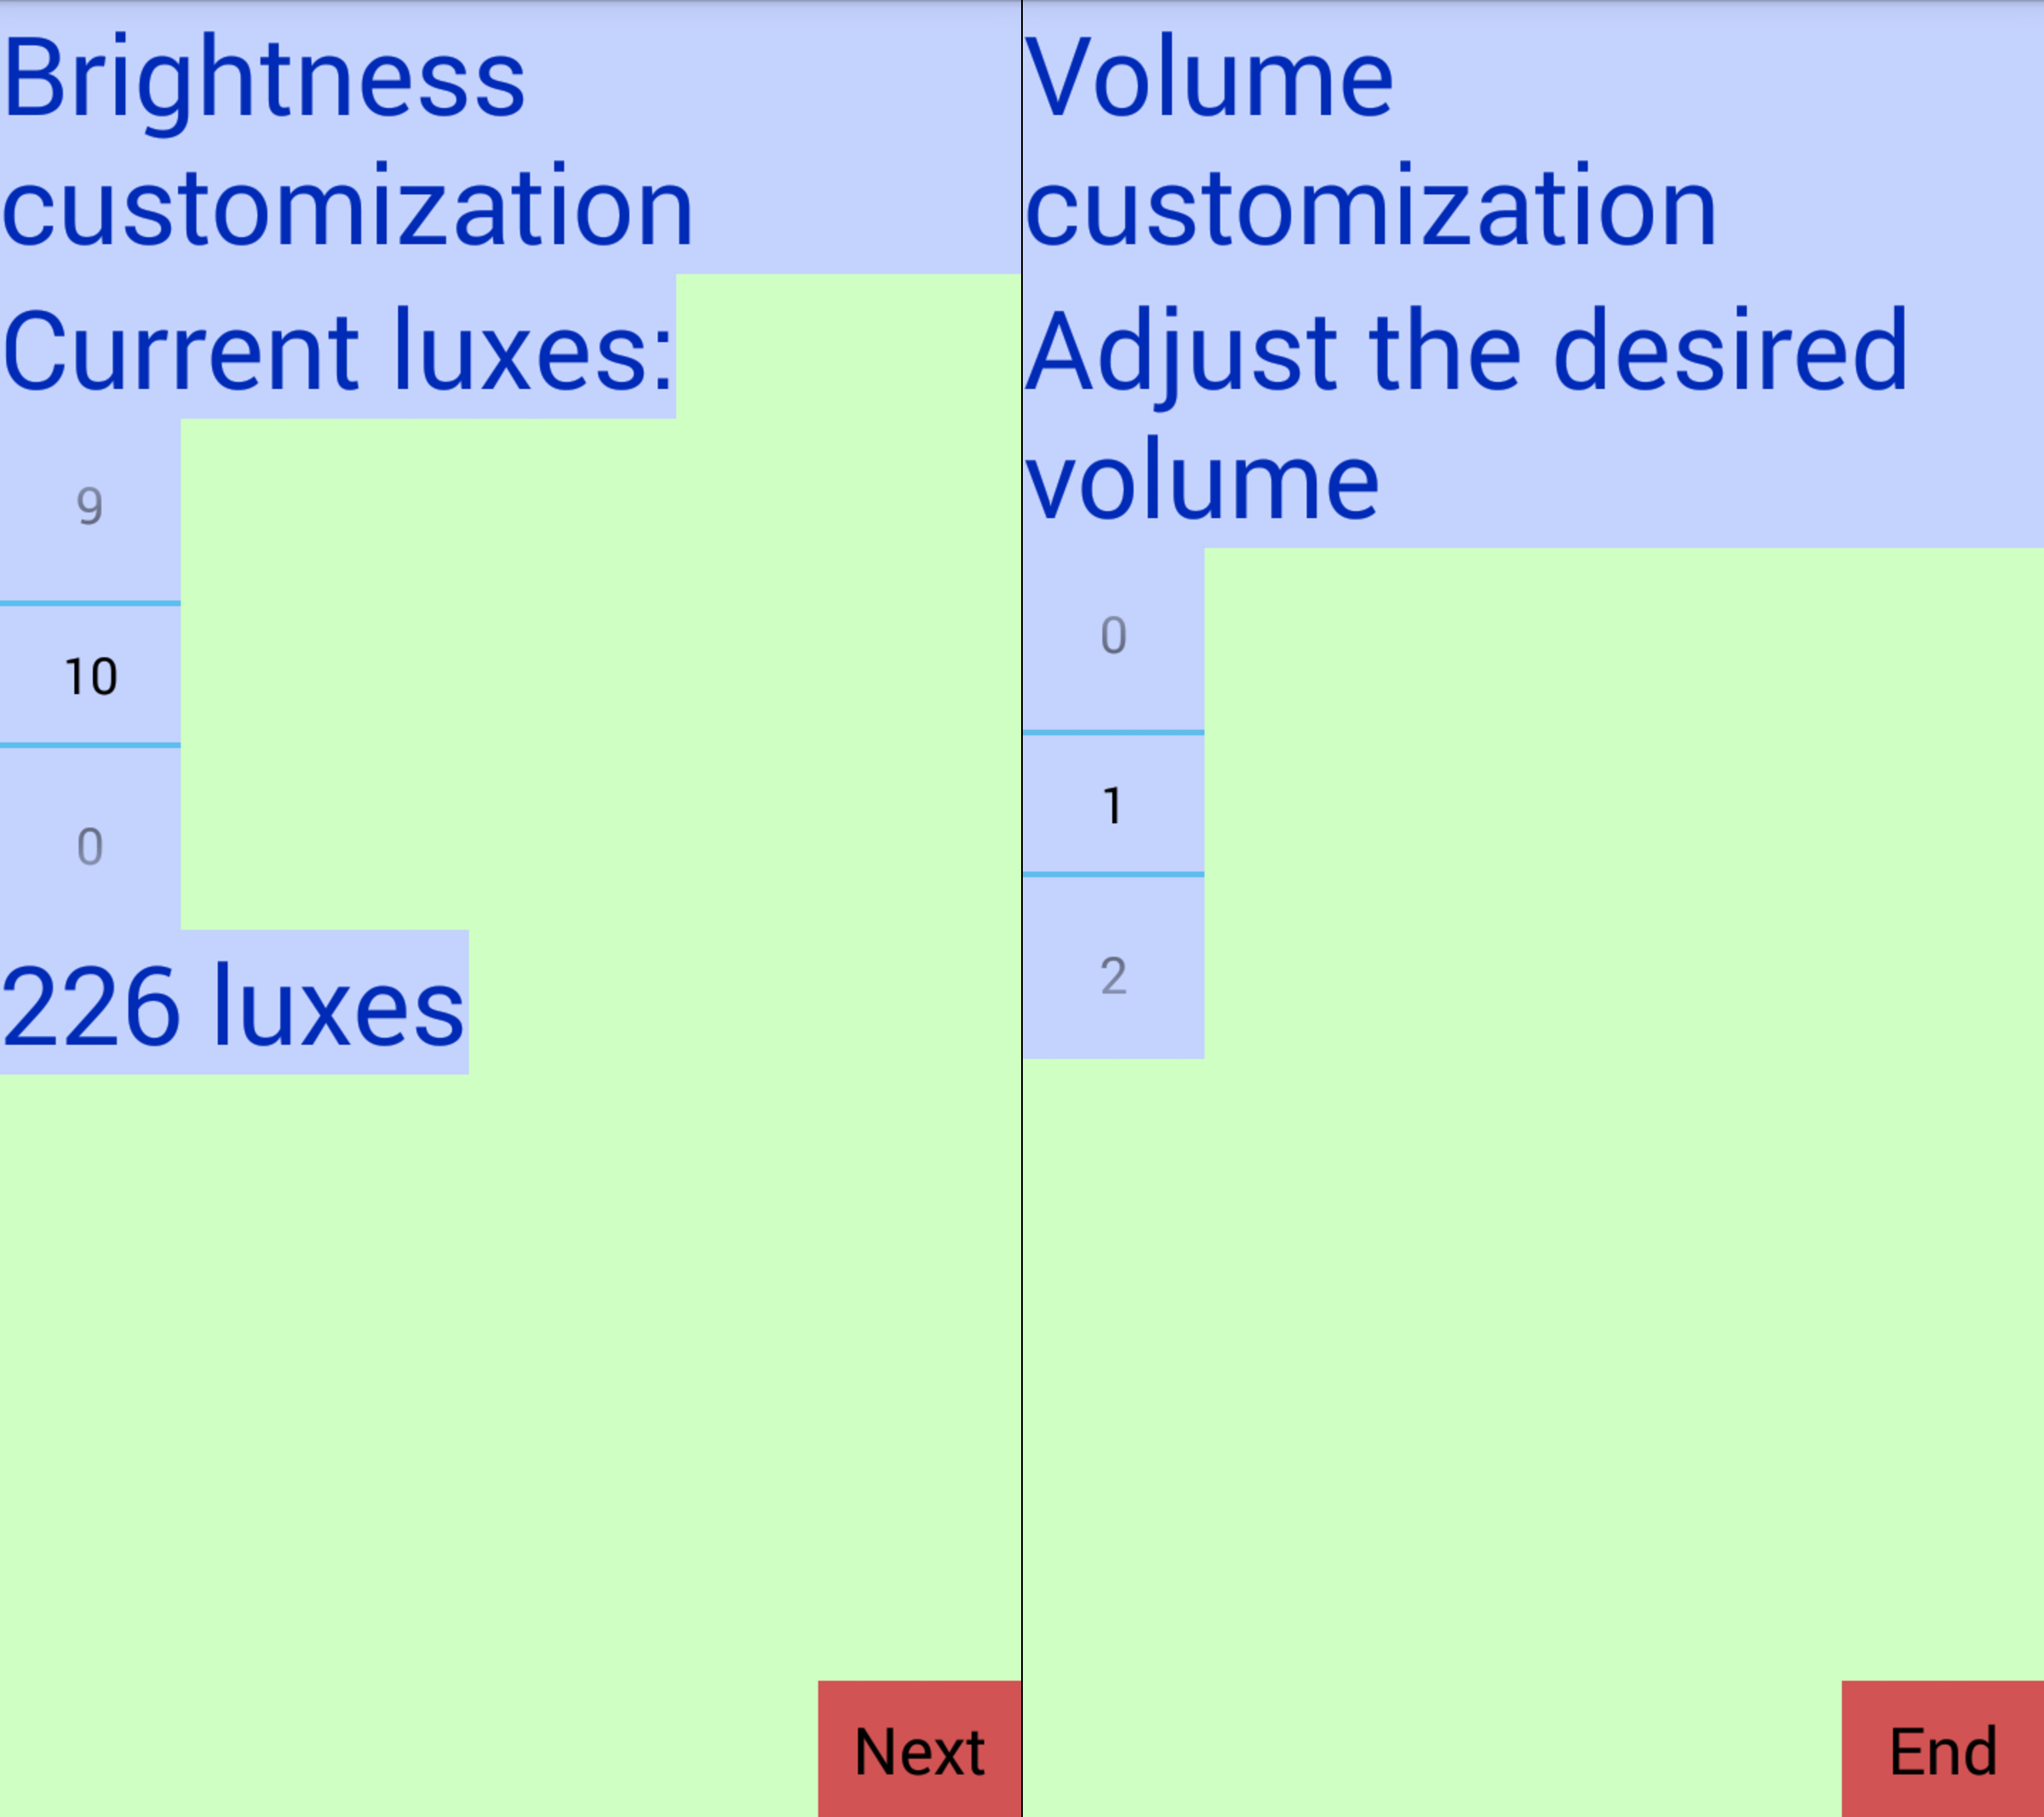
\includegraphics[width=0.50\textwidth]{context_activity.pdf}
\caption{Brightness (left) and Volume (right) adjustment sensing the surrounding
light and noise.}
\label{fig:context_activity}
\end{figure}


\subsubsection{The Device Characteristics}
\label{sec:device_characteristics}

Device characteristics are significant within the AdaptUI platform. These
characteristics limit the possible adaptations of the user interface. For example,
not all the smartphones have the same maximum brightness or sound levels, nor
they have the same connectivity capabilities. Thus, being aware of each device's
capabilities becomes essential in AdaptUI.

The device characteristics are collected by the Capabilities Collector by using
the \textit{Settings.System} class in Android. This class contains global
system-level device preferences. Listing~\ref{lst:device_settings_brightness} 
shows a piece of code which requests the maximum values for the brightness. To 
allow the user to change the brightness of the device's screen a NumberPicker 
element is shown. In its initialization, it is needed to specify the minimum and 
the maximum values of the range. Thus, the user is able to configure the brightness 
to $0$. For the maximum brightness value it is needed to state a default value 
of $1F$.

\inputminted[linenos=true, fontsize=\footnotesize, frame=lines]{java}{4_system_architecture/device_settings_brightness.java}
\captionof{listing}{Android NumberPicker initialization with a minimum value of 0 and a 
maximum value requested to the \textit{Settings.System class}.\label{lst:device_settings_brightness}}


On the contrary, to get values related to audio, the \textit{AudioManager} class
is required. 
% Listing~\ref{lst:device_settings_volume} shows a piece of code with
% which the developer initializes a NumberPicker with the minimum and maximum
% volume levels available in the current device.
% 
% \inputminted[linenos=true, fontsize=\footnotesize, frame=lines]{java}{4_system_architecture/device_settings_volume.java}
% \captionof{listing}{Android NumberPicker initialization with a minimum value of 0 and a 
% maximum value requested to the AudioManager class.\label{lst:device_settings_volume}}


Before asking the user about the way of interaction, the Capabilities Collector
performs an analysis about several device's capabilities. Several hardware
details are collected: processor maximum speed, processor availability, battery
current levels, maximum and current available memory, available input modes, 
and so forth. All the characteristics are shown in Table~\ref{tbl:device_characteristics}. 
These are stored during the process for the Semantic Modeller to store in the 
final model.

\begin{table}[H]
  \caption{Requested device characteristics.}
 \label{tbl:device_characteristics}
\footnotesize
\centering
 \begin{tabular}{l l}
  \hline 
  \textbf{Characteristic}& \textbf{Description}				\\
  \hline
  Brightness		& Describes the current device’s brightness.	\\
  Contrast		& Represents the current device’s contrast.	\\
  Volume		& Describes the current device’s volume.	\\
  Processor		& Models the number of the device’s cores.	\\
  OS version		& Indicates the current	\ac{os} version.	\\
  Acceleration		& Represents the current X, Y, Z acceleration.	\\
  Orientation		& Current orientation of the device.		\\
  Device memory		& Maximum device memory.			\\
  Available memory	& Current available device memory.		\\
  Battery		& Current device battery levels.		\\
  Screen resolution	& Maximum screen resolution.			\\
  Storage		& Maximum available storage.			\\
  Available storage	& Current available storage.			\\
  Processor		& Maximum processor of the device.		\\
  Available processor	& Current processor availability.		\\
  \hline
\end{tabular}
\end{table}


\subsection{The Semantic Modeller}
\label{sec:semantic_modeller}

Once the Capabilities Collector has finished its task, all the collected
knowledge is stored in the mobile. The Semantic Modeller's goal is to build a 
semantic representation of this knowledge through the AdaptUIOnt ontology and
store it in the mobile device. This task requires from a semantic reasoner. 
However, there are no available and remarkable reasoners written in Java and 
compatible with Android. Thus, an Android port of the 
Pellet~\citep{pellet} reasoning engine has been
developed: \textit{Pellet4Android}. As Pellet is available for open source
applications under the terms of the \ac{agpl} version 3 license, the provided
\textit{Pellet4Android} is also available in Github~\citep{pellet4android}
under the same license regulations.

During the following subsections both versions of the Pellet reasoning engine
are presented. First, in Section~\ref{sec:pellet}, the Java based Pellet reasoning
for desktop is introduced. Next, Section~\ref{sec:pellet4android} describes the
process followed to port Pellet to Android.

As the Semantic Modeller finishes storing the corresponding knowledge in the
AdaptUIOnt ontology, several rules are triggered. The main consequence of the
execution of these rules is shown through the \textit{Adaptation} class. This
class is filled with the adaptation values that will be requested by the
Adaptation Layer, which is the next layer of the AdaptUI architecture.


\subsubsection{Pellet}
\label{sec:pellet}

% \begin{description}
%   \item[\Defi{Reasoner by~\citet{owlapi_reasoners}}] \hfill \\
%   \begin{mdframed}[hidealllines=true,backgroundcolor=gray!20]
%   \textit{``A reasoner is a key component for working with \ac{owl} ontologies. 
%   In fact, virtually all querying of an \ac{owl} ontology (and its imports closure) 
%   should be done using a reasoner. This is because knowledge in an ontology 
%   might not be explicit and a reasoner is required to deduce implicit knowledge 
%   so that the correct query results are obtained''}~\citep{owlapi_reasoners}.
%   \end{mdframed}
% \end{description}

Developed by Clarkparsia, Pellet is a free and open source \ac{owl}-\ac{dl}
reasoner written in Java. As a \ac{dl} reasoner, it provides several standard 
inference services:

\begin{itemize}
  \item \textit{\ac{owl}-\ac{dl} consistency checking}: Pellet assures that the 
  knowledge represented in the ontology does not contain contradictory facts. 
  \citet{carroll_owl_2004} define that \textit{``an \ac{owl} consistency checker 
  takes a document as input, and returns one word being Consistent, Inconsistent, 
  or Unknown.''} In \ac{dl} terminology  this is the operation to check the 
  consistency of an ABox with respect to a TBox (see the description of this 
  \ac{dl} terminology in Table~\ref{tbl:dl_terms}).
  
  \item \textit{Concept satisfiability}: Determines whether it is possible for 
  a class to have any instances. This avoids cases in which unsatisfiable classes 
  might define instances, which will cause the ontology to be inconsistent.
  
  \item \textit{Classification}: Pellet is able to create the complete class 
  hierarchy from the computation of the subclasses relations between every 
  named class. This allows performing future queries (i.e., getting all the 
  direct subclasses of a class).
  
  \item \textit{Realization}: It is able to find the most specific classes that 
  an individual belongs to. Realization directly depends on classification, and 
  it cannot be done without it.
\end{itemize}


\begin{table}[H]
  \caption{Several \ac{dl} terminology.}
 \label{tbl:dl_terms}
\footnotesize
\centering
 \begin{tabular}{l l}
  \hline 
  \textbf{Component} 		& \textbf{Description}				\\
  \hline
  ABox (Assertional Box)	& Contains assertions about individuals	\\
				& (i.e., \ac{owl} facts such  as type, property	\\
				& -value, equality or inequality assertions).	\\
  TBox (Terminological Box)	& Contains axioms about classes, i.e., \ac{owl}	\\
				& axioms such as subclass, equivalent class 	\\
				& or disjointness axioms.			\\
  \acl{kb}			& A combination of ABox and TBox (i.e.,		\\
				& a complete ontology).				\\
  \hline
  
\end{tabular}
\end{table}

The reasoning capabilities of Pellet are accessible through different interfaces.
For example, Pellet is directly integrated with the Protégé ontology 
editor~\citep{protege}. Thus, reasoning capabilities
are allowed through the user interface of this editor. For developers, there are
several tools provided as \acsp{api} which allow the utilisation of Pellet. The
most significant ones are Apache Jena~\citep{jena}
and Manchester \ac{owl}-\ac{api}~\citep{owlapi}:

\begin{itemize}
  \item Jena: Apache Jena (or Jena) is a free and open source framework written
  in Java which allows building semantic web and Linked Data applications. The
  framework is composed of different \acp{api} interacting together to process 
  \ac{rdf} data.
  
  \item \ac{owl}-\ac{api}: Available under \ac{lgpl} or Apache Licenses, the 
  \ac{owl}-\ac{api} is an open source high level \ac{api} maintained by the 
  University of Manchester for working with \ac{owl} ontologies. Closely aligned 
  with the \ac{owl} 2 structural specification, the \ac{owl}-\ac{api} supports 
  parsing and rendering in the syntaxes defined in the \ac{w3c} specification 
  (i.e., Functional Syntax, \ac{rdf}/\ac{xml}, \ac{owl}/\ac{xml} and the 
  Manchester \ac{owl} Syntax), the manipulation of ontological structures, and 
  the use of reasoning engines (i.e., Chainsaw, FaCT++, JFact, HermiT, Pellet 
  and RacerPro).  
\end{itemize}

% The core of the system is the tableaux reasoner. This reasoner checks the
% consistency of a knowledge base and allows Pellet to support \ac{swrl}~\citep{swrl}
% rules language.


\subsubsection{Reasoning with Pellet in Android: Pellet4Android}
\label{sec:pellet4android}

The AdaptUI platform was conceived to support reasoning and semantic knowledge
representation due to the benefits that ontologies bring. Nevertheless, after
analysing the possibilities and solutions provided by the community (i.e., mobile
reasoning platforms) we found that, although nowadays mobile capabilities allow
heavier processing, there are no remarkable efforts in the area.

\citet{yus_android_2013} noticed this issue and made great efforts porting
several Java based reasoners to Android. Although the authors do not provide the
developed ports to the community, they provide several instructions to make these
reasoners available for Android devices. Thus, following these instructions a port
of Pellet has been developed for AdaptUI: \textit{Pellet4Android}.

As Pellet, \textit{Pellet4Android} also supports full \ac{owl} 2 and \ac{dl} 
rules. To make Pellet run in Android the following steps were needed:

\begin{itemize}
  \item Pellet uses Jena, which is a free and open source framework written in
  Java which allows building semantic web and Linked Data applications. However,
  Jena is not directly importable to Android. Thus, it is necessary to replace it
  with Androjena~\citep{androjena}. Androjena
  is a porting of Hewlett-Packard's Jena semantic web framework to Android. 
  
  \item Pellet also imports the \ac{jaxb} library~\citep{jaxb} for \ac{xml} 
  parsing. \ac{jaxb} is able to translate \ac{xml} Schemas building a set of 
  classes that correspond to that schema. It originally comes with the Java 1.6 
  release, but its easily importable to previous Java version integrating the 
  \ac{jaxb} jar files. The problem is that \ac{jaxb} uses classes that are not 
  compatible with Android. Thus, this package has been removed. 
  
  \item As the official Oracle documentation states, the \textit{javax.xml.bind}
  package \textit{``provides a runtime binding framework for client applications
  including unmarshalling, marshalling, and validation capabilities''}~\citep{javax_xml_bind}.
  Nevertheless, this package is also incompatible with Android, and we should
  remove it from the package list and the build path.
  
  \item Also related with the way Java manages \ac{xml} files, the 
  \textit{org.apache.xerces}~\citep{xerces} package
  is used for the creation and maintenance of \ac{xml} parsers and related
  software components. Several classes under this package are not importable by
  Android, so the package has to be removed.
  
  \item Finally, under the \textit{com.clarkparsia.pellet} package there are several
  classes that are not directly importable by Android. Thus, without removing them,
  we have to search the specific troublesome lines of code (usually related with
  concrete data types and exceptions) and comment them. 
\end{itemize}

Figure~\ref{fig:pellet4android} shows the package structure of the
\textit{Pellet4Android} port and the imported libraries in the Android project.
% 
% \InsertFig{pellet4android}{fig:pellet4android}{Package structure (left) and 
% needed libraries (right) for Pellet4Android}{}{0.85}{}

\begin{figure}[H]
\centering
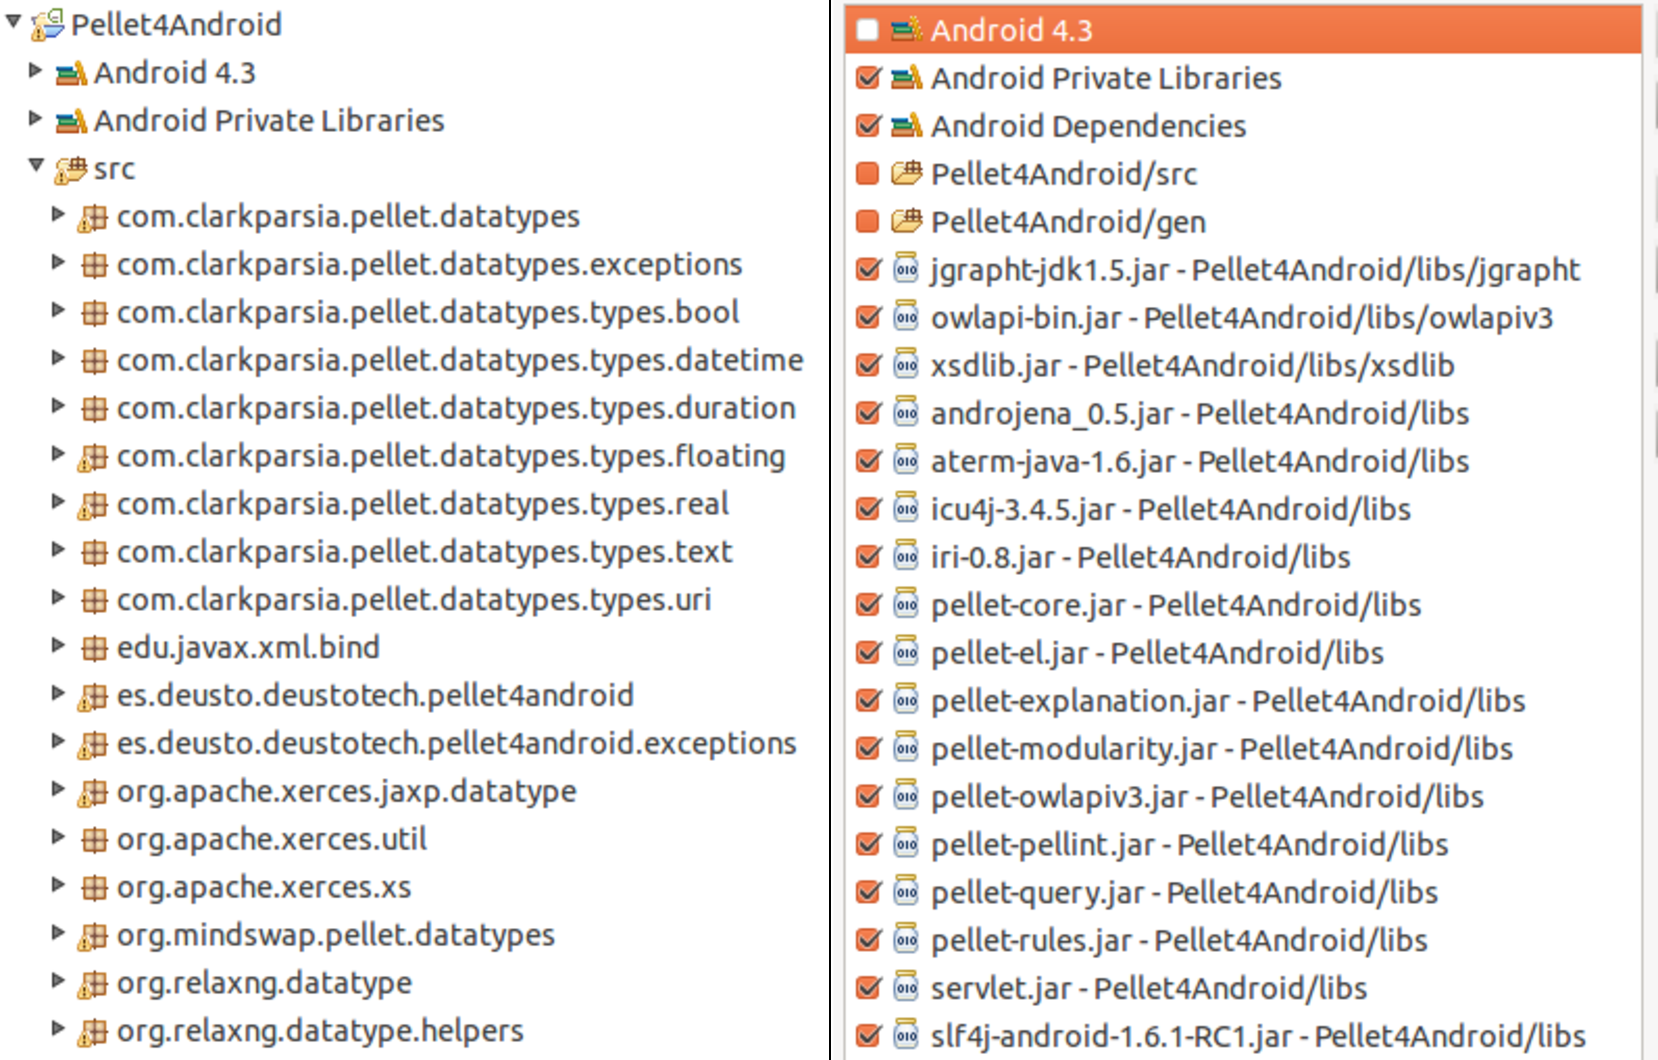
\includegraphics[width=0.85\textwidth]{pellet4android.pdf}
\caption{Package structure (left) and needed libraries (right) for Pellet4Android.}
\label{fig:pellet4android}
\end{figure}


As~\citet{yus_android_2013} remarked, it is important to provide a larger heap
size. To do this, the \textit{android:largeHeap} tag of the AndroidManifest.xml 
file of the project has to be changed to \textit{true}.

A first evaluation of the port was carried out by~\citet{yus_android_2013}.
Nevertheless,~\citet{bobed_android_2014} performed a second evaluation of the
Pellet version for Android obtaining promising results in terms of efficiency
and time responsiveness. Although in this dissertation a similar approach to port 
Pellet has been followed, it is impossible to be a 100\% sure if the results are 
the same (as the version by~\citet{yus_android_2013} was not available for testing). 
Thus, in Chapter~\ref{cha:evaluation} an evaluation of \textit{Pellet4Android} is 
included.

